%--------------------------------
%--------------------------------
\chapter{Implementierungsdetails}
\label{chapter:implementation_detail}


%----------------------------
\section{Aufbau der Software}
% Erweiterbarkeit?

Die Implementierung wurde mit der Programmiersprache Java durchgeführt. In Abbildung \ref{classDiagram} ist der Programmaufbau stark vereinfacht dargestellt. Das Diagramm ist an UML-Klassendiagramme angelehnt. Pfeile stehen jedoch nicht für Teilbeziehungen oder Vererbung, sondern für den Datenfluss.\\
Aus der Benutzeroberfläche (GUI) werden die Benutzereingaben ausgelesen. Diese gehen dann einerseits als Bedingungen in die PCA ein und andererseits sind sie Zusatzeingaben für die Skelettgenerierung (\zb die Anzahl der Flossen). 
Über den "`PcaDataReader"' werden die Beispiele für die PCA eingelesen und der "`PcaHandler"' verwaltet alles was mit der PCA zu tun hat.\\
Die zentrale Komponente ist der "`SkeletonGenerator"'. Er ist dafür verantwortlich die Einzelteile des Skeletts zu generieren. Zu jedem Zeitpunkt hält er alle terminalen und nichtterminalen Elemente. Die Ersetzungsregeln der Grammatik sind im "`RuleDictionary"' und die Parameter für die Grammatik in "`SkeletonMetaData"' gespeichert. Die Klasse "`SkeletonMetaData"' implementiert das "`Serializable"' Interface \cite{JavaSerialization} und wird, wenn ein Skelett gespeichert werden soll, als Textdatei herausgeschrieben (siehe Abschnitt \ref{load_skeletons}).\\
Sind alle Einzelteile generiert, werden alle zu spiegelnden Elemente mit der Methode "`calculuateMirroredElements()"' gespiegelt. Das fertige Skelett geht dann an den "`ObjGenerator"', der ein 3D-Modell mit Hilfe der 3D-Modelle aus der "`BoneLibrary"' erstellt.

\begin{figure}
 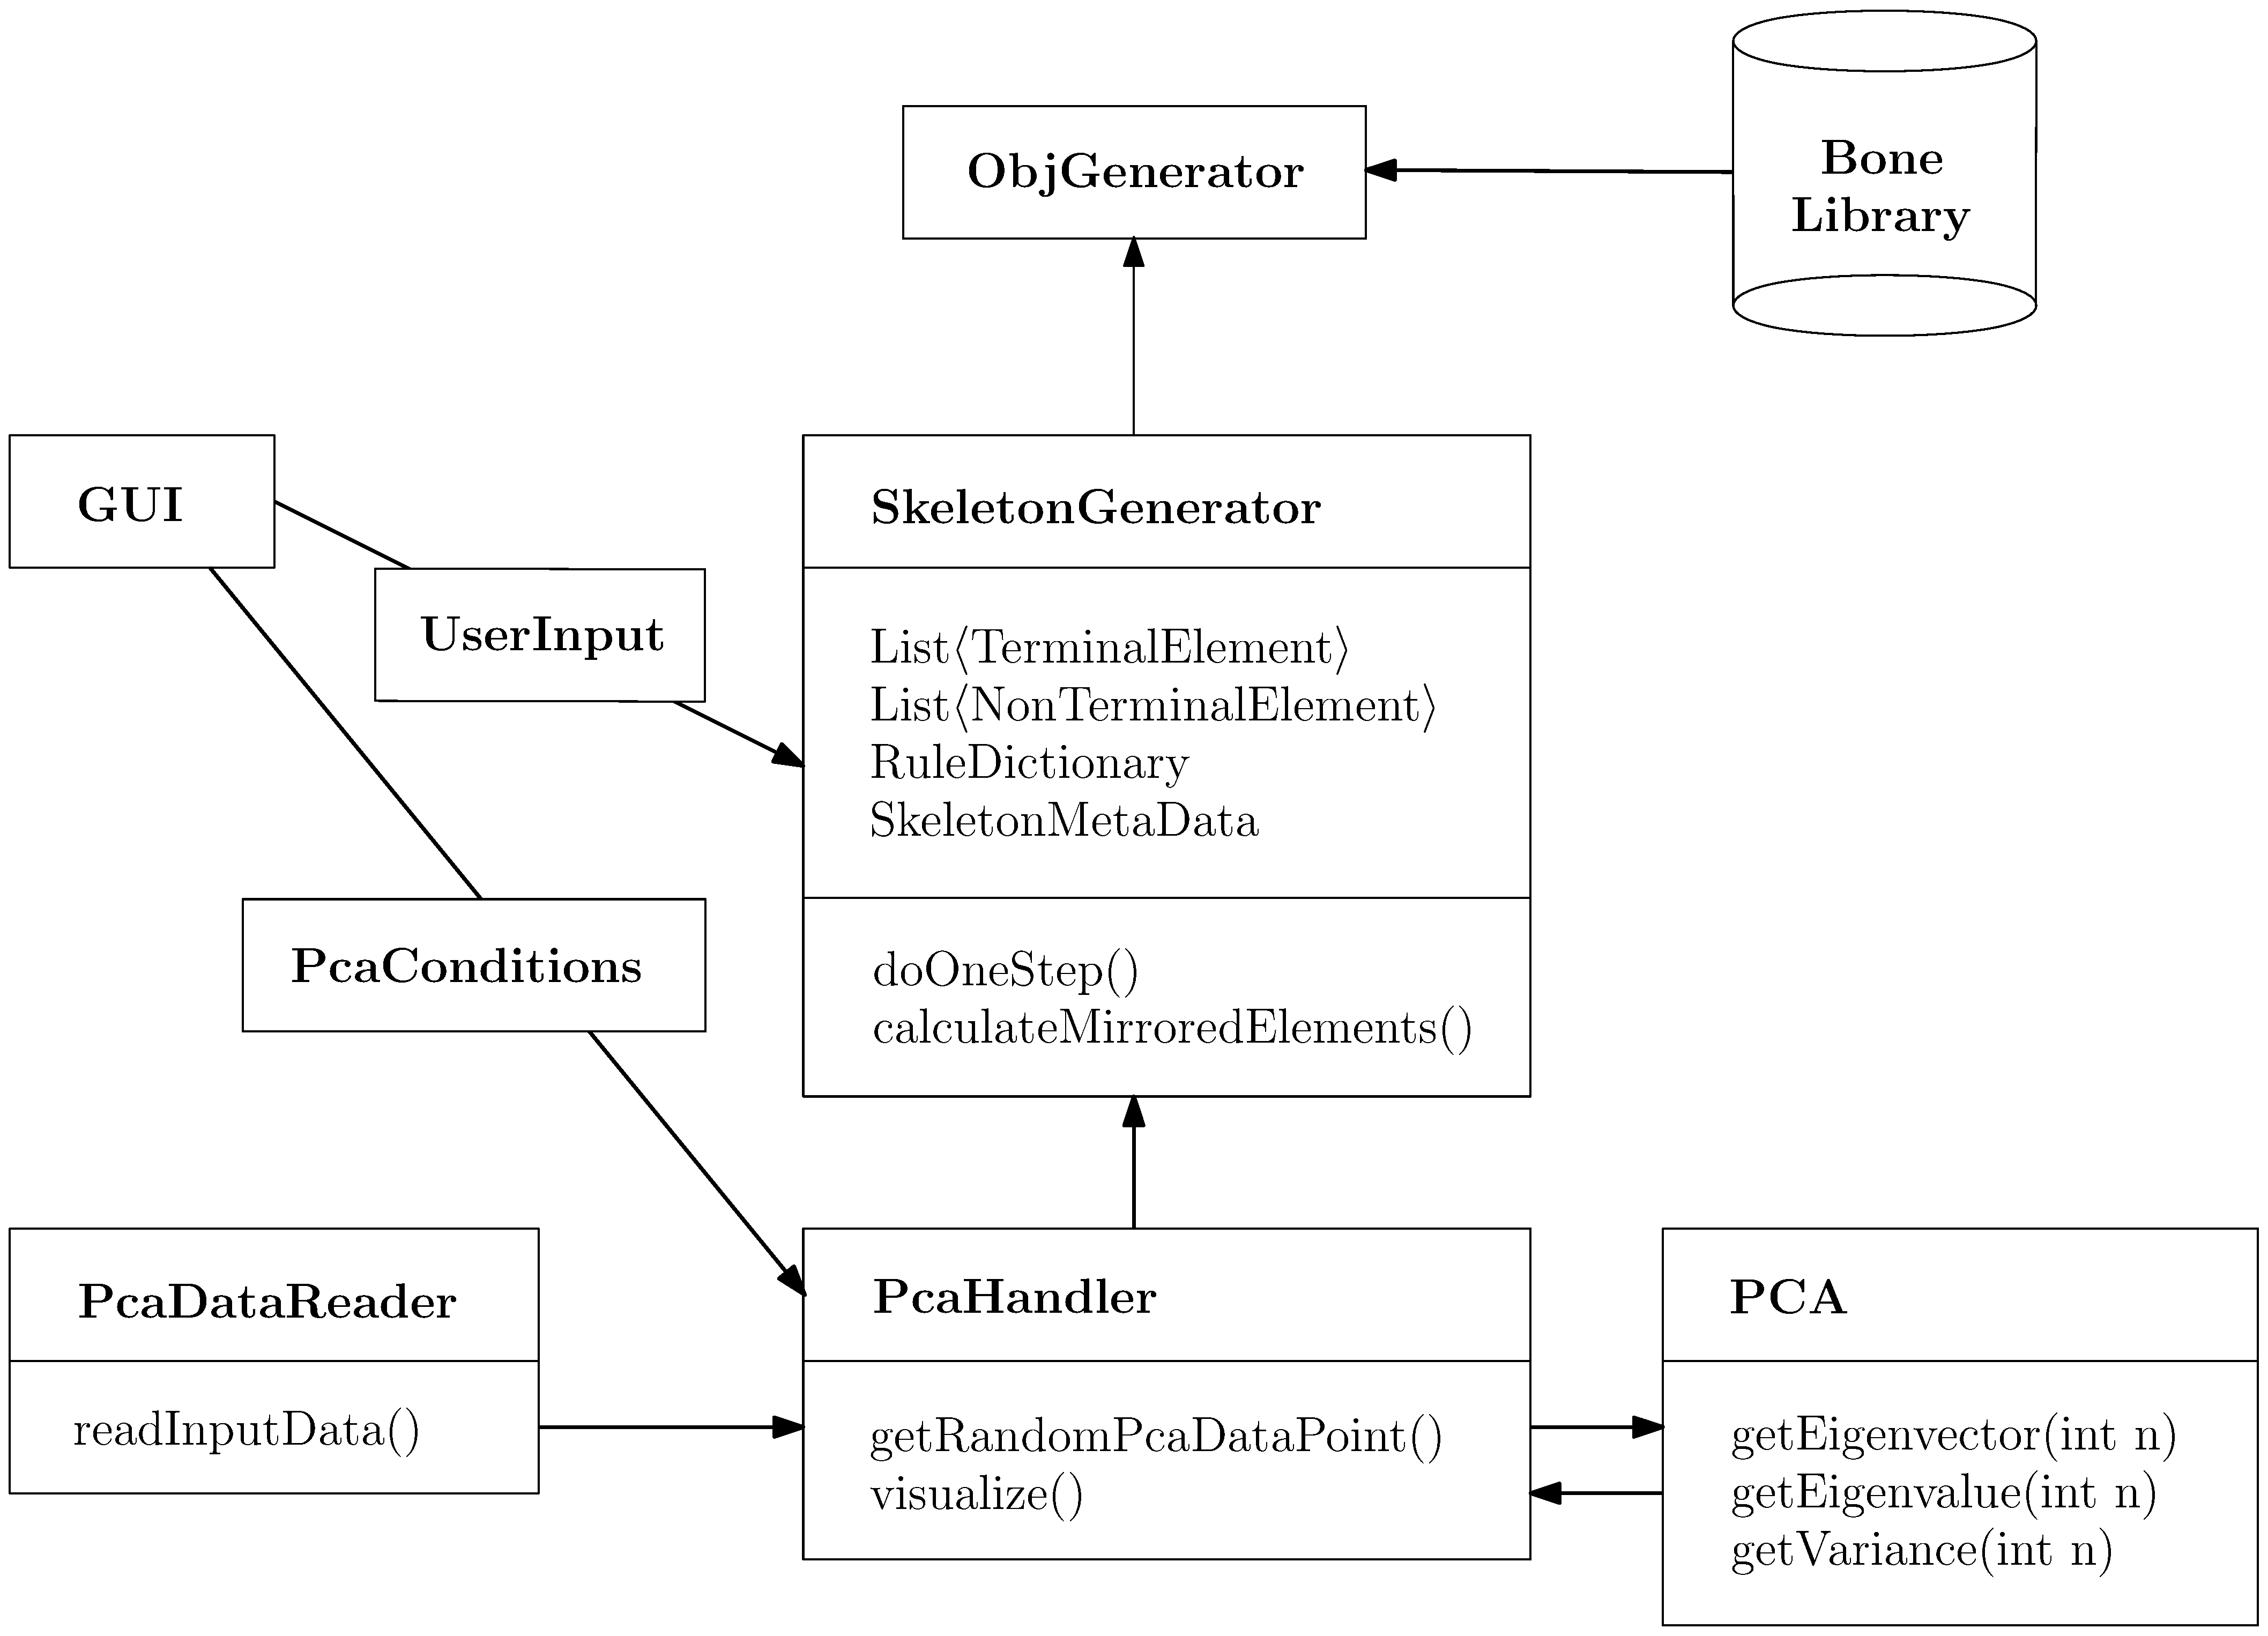
\includegraphics[width=\textwidth]{graphics/classDiagram}
 \caption{Stark vereinfachte Darstellung der Softwarearchitektur. Jeder Kasten steht für eine Klasse, wie in UML-Klassendiagrammen. Pfeile sollen den Datenfluss darstellen.}
 \label{classDiagram}
\end{figure}


%------------------------------------
\section{Dateiformate für 3D-Modelle}

Das einfachste Format zur Darstellung von 3D-Objekten ist das offene Dateiformat Wavefront OBJ \cite{obj}. Es kann nur geometrische Formen speichern, keine zusätzlichen Informationen wie \zb Gelenke und deren Einschränkungen.\\
Andere weit verbreitete Formate sind FBX von Autodesk \cite{fbx} und Alembic \cite{alembic}. Sie bieten mehr Möglichkeiten als OBJ, sind aber auch ungleich aufwändiger programmatisch zu erzeugen.

Um das 3D-Modell des erzeugten Skeletts zu speichern reicht das OBJ-Format aus. Zur Weiterverarbeitung, \zb für Animationen, können die Daten dann leicht in das benötigte Dateiformat umgewandelt werden. Für das Laden und Schreiben von OBJ-Dateien wird die Java-Bibliothek Obj \cite{ObjLoader} verwendet.
Sollten in Zukunft zusätzliche Daten exportiert werden können, müsste neu evaluiert werden welches Dateiformat am besten geeignet ist.


% \begin{itemize}
%  \item Jeder Editor geht mit Muskeln und Gelenken anders um. Gibt es ein Dateiformat, das nicht speziell zu einem Editor gehört, dass Bedingungen an die Rotation von Gelenken speichern kann?
%  \item Eigenes Format erzeugen? Dann bräuchte man Plugins um es in verschiedenen Editoren laden zu können. Viel verwendeter Editor: Houdini (kostenlos für Studenten aber nicht Open Source). Oder selbst darstellen (siehe Interaktivität).
% \end{itemize}


%--------------------------------
\section{Transformationsmatrizen}
\label{implementation_detail_matrices}

\todo{Recherchiere warum rechtshändige Koordinatensysteme bzw. konsistene Koordinatensysteme wichtig sind (back face culling, Rotationsrichtung der Matrizen bei positiven Winkeln)}

Jedes Element im Skelett speichert, relativ zu seinem Elternelement, die Position des Ursprungs seines Koordinatensystems. Um den Überblick über die Transformationsmatrizen bzw. Abbildungen behalten, die vom einen ins andere Koordinatensystem umwandeln, hier zwei Übersichtsgrafiken:
\todo{Erzeugung von Elementen auf der Wirbelsäule mit gegebener Weltposition + gespiegelte Elemente}

\begin{figure}
 \centering
 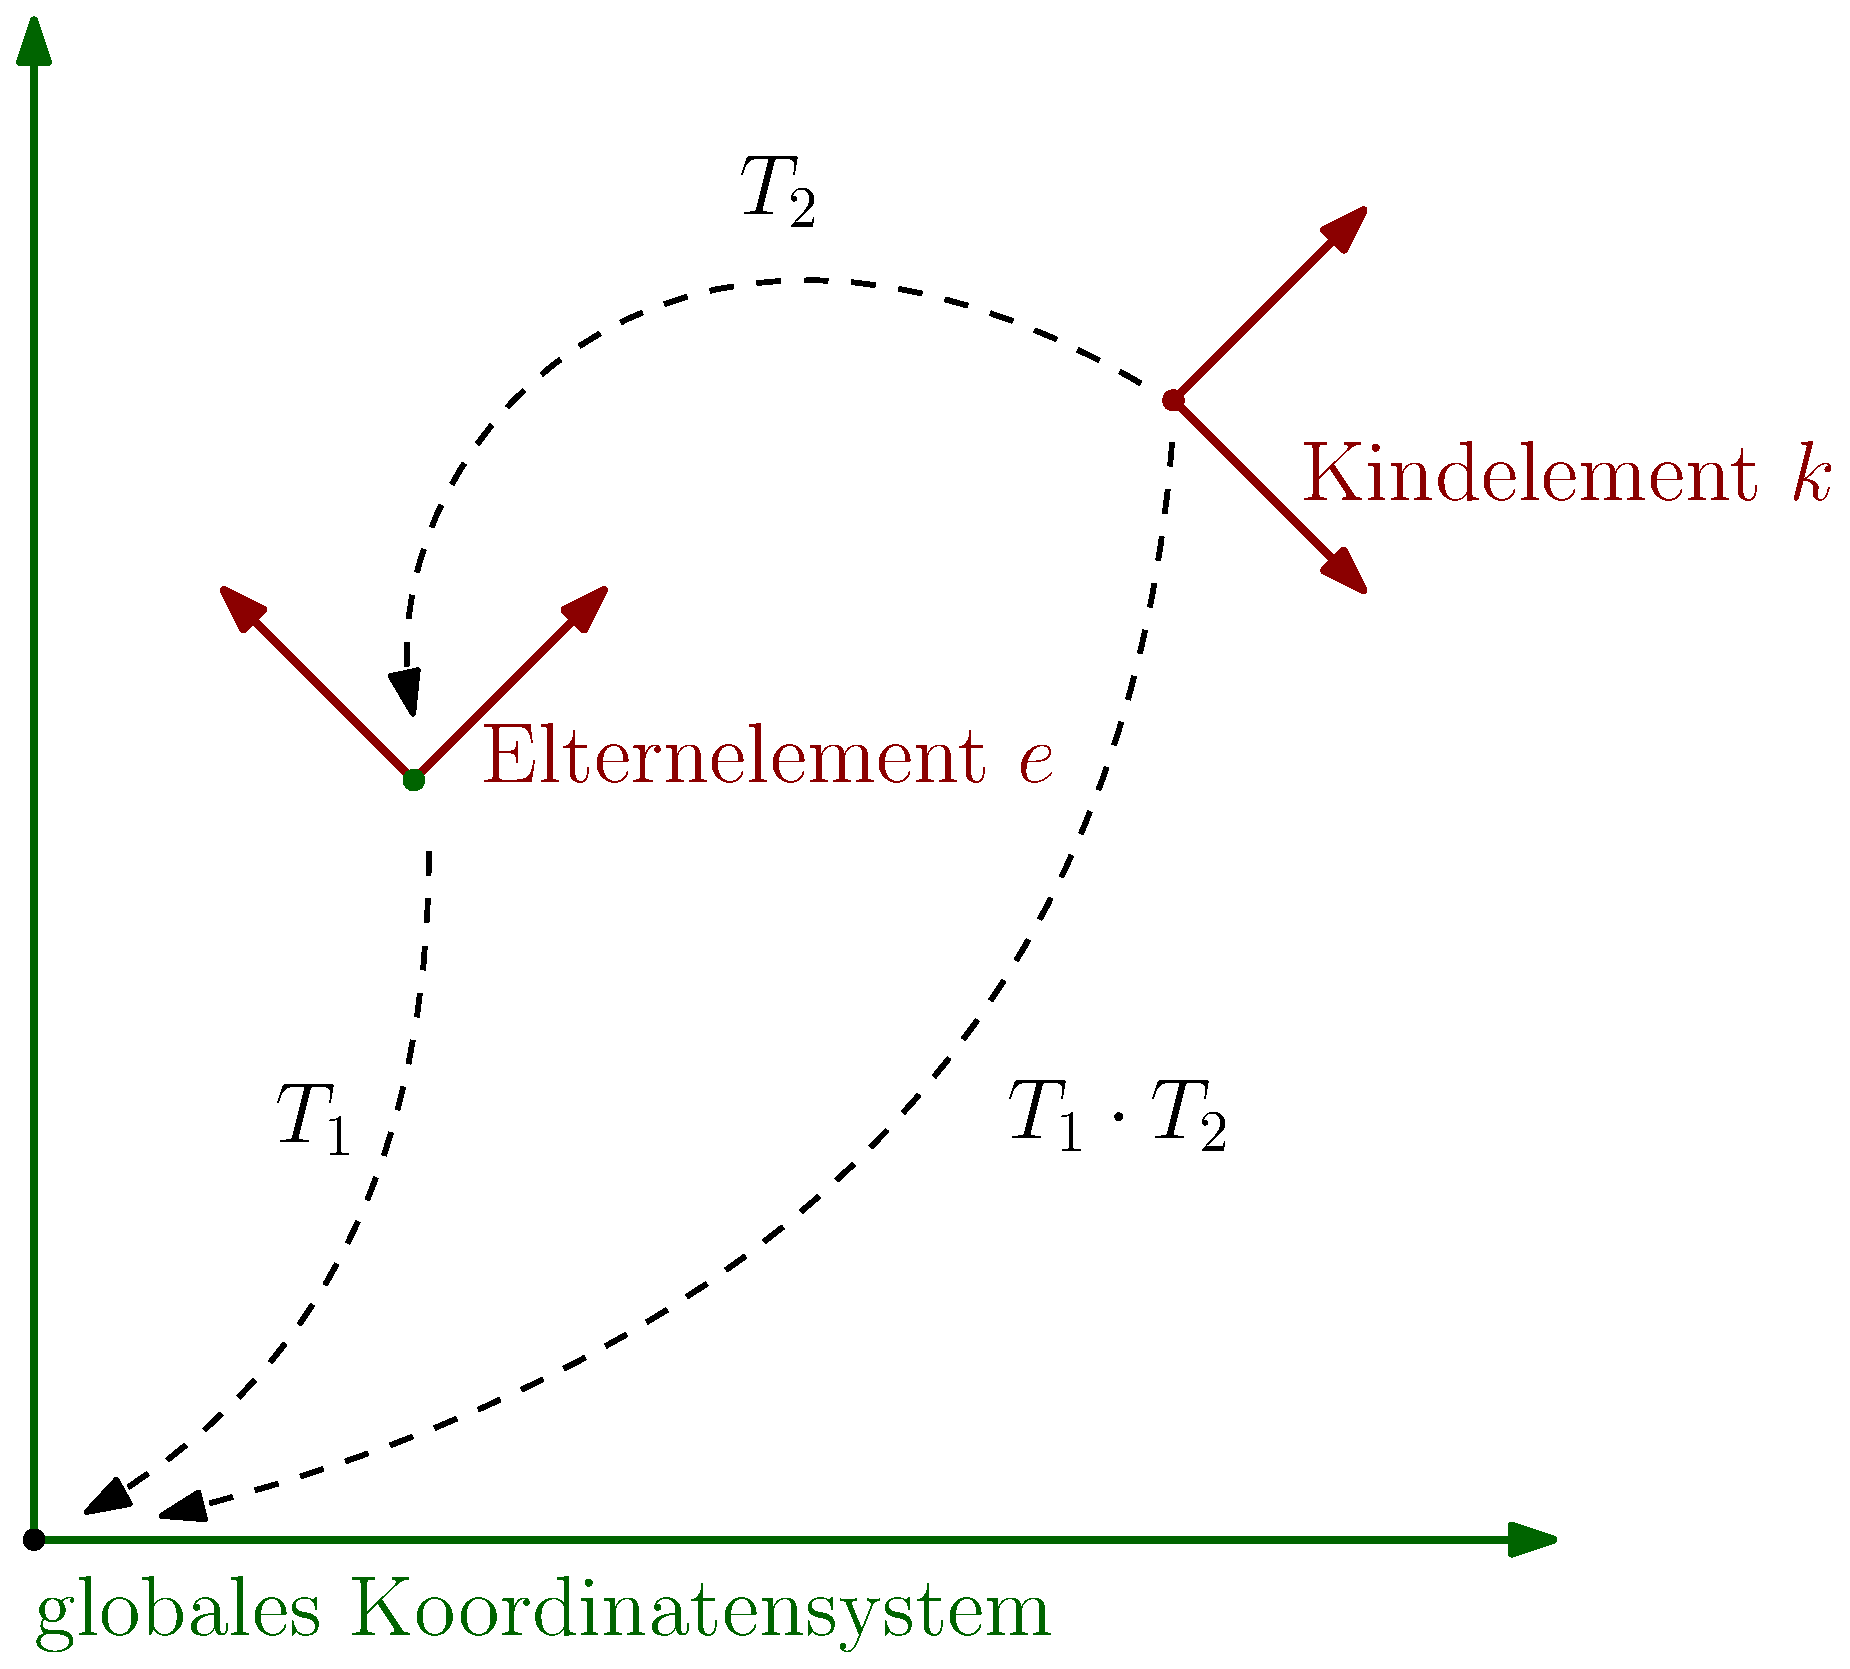
\includegraphics[width=0.6\textwidth]{graphics/transformation_matrices.eps}
 \caption{Gegeben sei das Element $e$. Die Abbildung, die die lokalen Koordinaten von $e$ in globale Koordinaten umrechnet sei $T_1$.
 Jedes Kindelement $k$ von $e$ speichert eine Transformationsmatrix $T_2$, die angibt wo der Ursprung des Koordinatensystems von $k$ relativ zum Koordinatensystem von $e$ liegt. Will man nun Koordinaten von $k$ in globale Koordinaten umrechnen, benötigt man die Abbildung $T_1 \cdot T_2$.}
\end{figure}

\begin{figure}
 \centering
 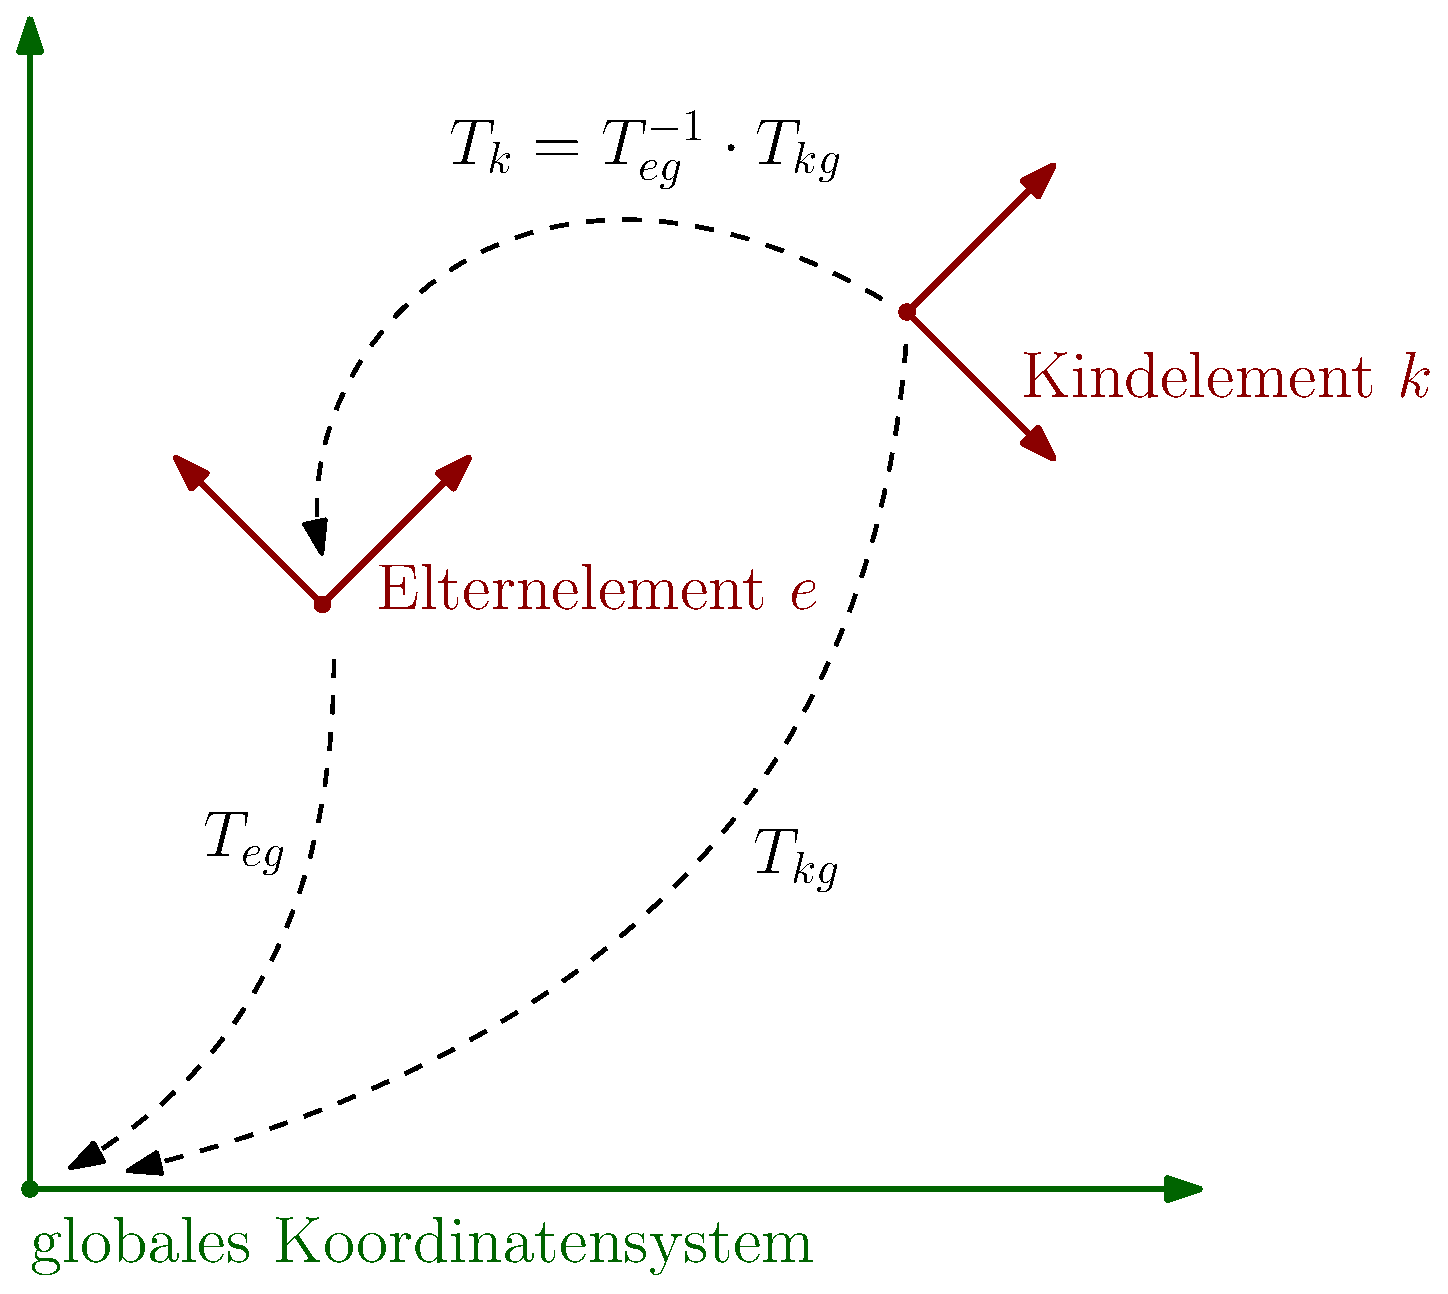
\includegraphics[width=0.6\textwidth]{graphics/transformation_matrices_spine.eps}
 \caption{Will man ein Element $k$ erzeugen, das Kindelement von $e$ ist und dessen globale Koordinaten bekannt sind, muss man die Abbildung berechnen, die die relative Position von $k$ angibt. Seien $T_1$ und $T_2$ jeweils die Transformationen in das globale Koordinatensystem von $e$ \bzw $k$. Dann ist die gesuchte Abbildung $T_1^{-1} \cdot T_2$.}
\end{figure}


%------------
\section{PCA}
\label{implementation_detail_pca}

Die Bilder der Skelette wurden folgendermaßen für die Datenerhebung vorbereitet:
 
 \begin{enumerate}
  \item Zuschneiden des Bildes, so dass möglichst nur das Skelett mit wenig Rand außen herum zu sehen ist.
  \item Einfügen in eine $1000 \times 1000$ Pixel große Bildumgebung.
  \item Verschieben innerhalb der Bildumgebung an den unteren Rand und horizontal in die Mitte.
 \end{enumerate}

 Ist das geschehen kann die Lage der Wirbelsäule und die Länge der Knochen der Extremitäten annotiert werden.
 
%- - - - - - - - - - - - - - - - -
\subsection{Annotation der Bilder}

Die Annotation der Bilder wurde per Hand mit dem Programm Inkscape\footnote{Programm zum erstellen und bearbeiten von Vektorgrafiken, \url{https://inkscape.org/de}} durchgeführt. Für jedes zu markierende Element wurde eine Strecke oder eine Bézierkurve eingefügt und mit einem vorher festgelegten Namen benannt. Diese Elemente wurden dann durch Inkscape als Pfade in der erzeugten svg-Datei gespeichert. Aus dieser Datei wurden dann automatisiert die eingetragenen Pfade mit ihren Koordinaten ausgelesen.

Folgende Details sind wichtig zu beachten, damit dieser Vorgang reibungslos abläuft. 
\begin{itemize}
 \item Man kann in Inkscape einstellen, dass Koordinaten immer absolut angegeben werden. Das ist sinnvoll um die Koordinaten leichter auslesen zu können.
 \item Der Ursprung des Koordinatensystems in Inkscape ist unten links, im svg-Format ist er aber oben links.
 \item Ebenen sollten in Inkscape nicht verschoben sein, sonst verschieben sich mit ihnen auch die Koordinaten.  
\end{itemize}

%- - - - - - - - - - - - - - - - - - - - - - - - - - - - - - - -
\subsection{Anpassung der PCA-Ergebnisse zur Weiterverarbeitung}

\begin{itemize}
 \item Um Wirbelsäule aus PCA Daten differenzierbar zu machen, wurden jeweils der vorletzte und der zweite Punkt von Hals und Rücken \bzw Rücken und Schwanz um den Kontaktpunk um den gleichen Winkel in gegensätzliche Richtungen gedreht, damit beide Bézierkurven an dem Kontaktpunkt die gleiche Steigung haben. \todo{beste Lösung?}
 \item An den Kontakpunkten der Wirbelsäulenteile ist die Steigung nicht unbedingt gleich (die Wirbelsäule als ganzes ist nicht $C^1$). Deshalb müssen vor der Weiterverwendung die jeweils nächsten Kontrollpunkte nach dem Kontakpunkt verschoben werden. Das wurde hier so gemacht, dass die zu verschiebenden Kontrollpunkte um den Kontakpunkt in gegensätzliche Richtungen rotiert wurden. Beide werden um den gleichen Winkel rotiert (siehe Abbildung \ref{smooth_spine}). Grundsätzlich könnten die Kontrollpunkte beliebig auf der Tangente des Kontaktpunkts platziert werden (rot im Bild) um eine übereinstimmende Steigung zu bekommen. Um den Verlauf der Wirbelsäulenteile möglichst wenig zu verändern ist es von Vorteil auch die Kontrollpunkte möglichst wenig zu verschieben. Man könnte die Punkte \zb auch senkrecht auf die Tangente projizieren. Welches Verfahren angewendet wird, ist jedoch nicht von großer Bedeutung. 
\end{itemize}

\begin{figure}
 \subfloat[vorher]{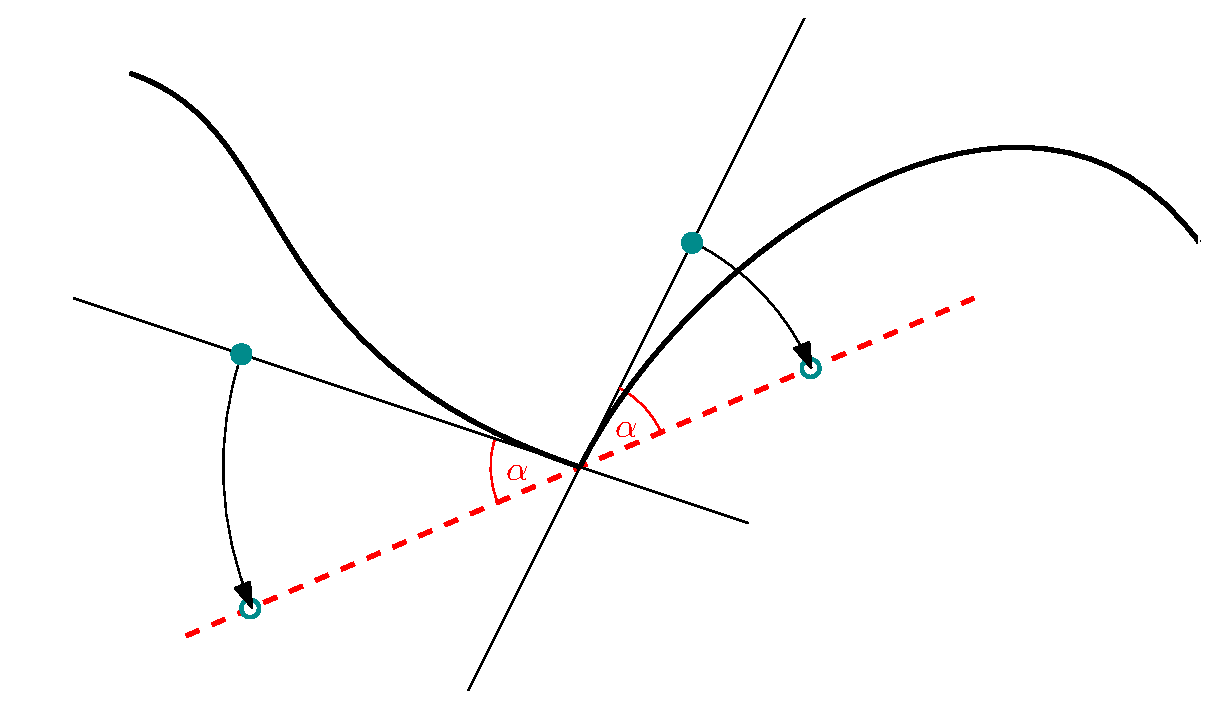
\includegraphics[width=0.5\textwidth]{graphics/smooth_spine1.eps}}
 \qquad
 \subfloat[nachher]{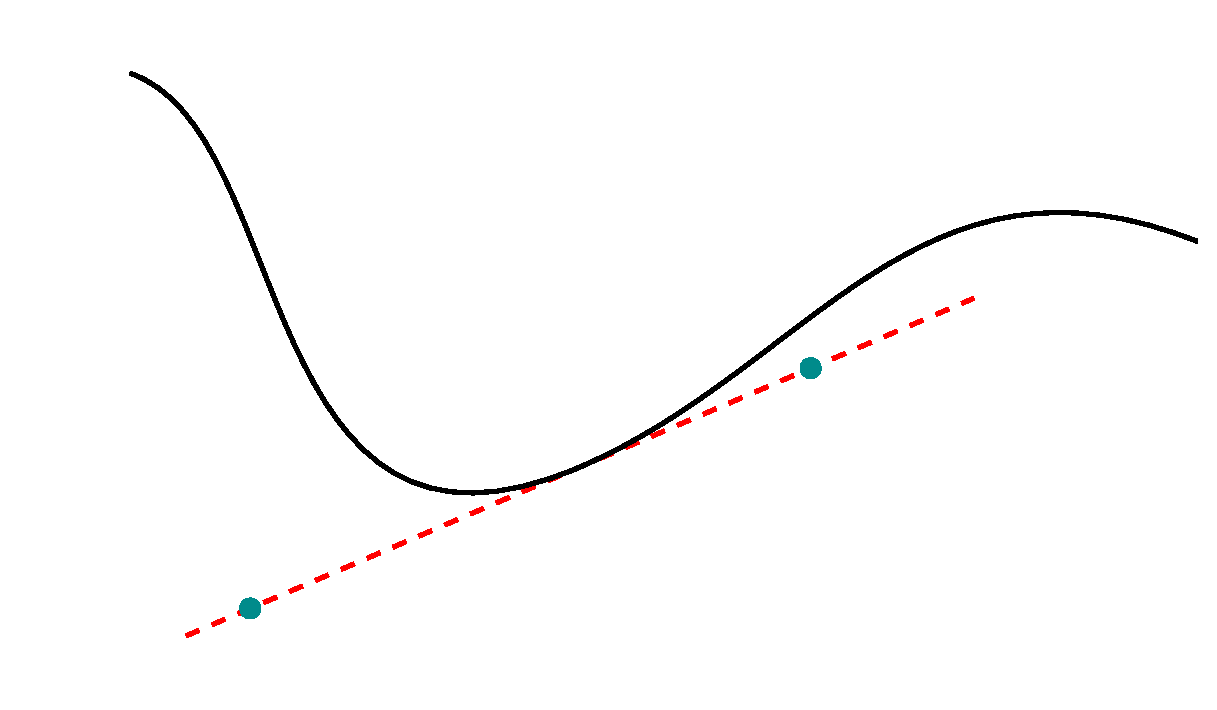
\includegraphics[width=0.5\textwidth]{graphics/smooth_spine2.eps}}
 \caption{Anpassung der Kontrollpunkte der Wirbelsäulenteile, wenn die Steigung an den Kontakpunkten ungleich ist. Die beiden Teile der Wirbelsäule und die Steigung am Kontaktpunkt sind hier in schwarz dargestellt. Die zu drehenden Kontollpunkte in cyan. In rot ist die resultierende Steigung und der Winkel, der für die Drehung verwendet wird, zu sehen.}
 \label{smooth_spine}
\end{figure}


%----------------------------------------------------------
\section{Probleme der Beinpositionierung bei kurzen Beinen}
\label{leg_positioning_short_legs}

Wie in Absatz \ref{leg_algo} zur Ausrichtung der Beine bereits beschrieben, treten bei sehr kurzen Beinen ein paar Probleme auf. Diese werden im Folgenden kurz umrissen.

\begin{enumerate}
 \item % Bodenhöhe nicht von Gelenk aus gemessen
   Bei Berechnung der Bodenhöhe wird die Beinlänge von den entsprechenden Kontrollpunkten der Bézierkurve aus gemessen, da die Position der Hüfte/Schulter in diesem Stadium noch nicht klar ist. Deshalb kann es bei sehr kurzen Beinen sein, dass der Abstand zwischen Boden und Gelenk zu groß ist und der Boden nicht erreichbar ist.
   
   In diesem Fall wird das Bein einfach komplett ausgestreckt senkrecht nach unten positioniert. Da der Abstand zwischen dem Hüft- / Schultergelenk und dem Kontrollpunkt der Bézierkurve nicht sehr groß ist, ist auch der Abstand zu Bodenhöhe nicht enorm und fällt nicht allzusehr auf.
   
 \item % keine starke Änderung durch Drehung der Gelenke
   Bei sehr kurzen Knochen ändert sich der Abstand zum Boden durch Drehung der Gelenke nicht so stark wie bei langen Knochen. Wenn der Winkel sich zu wenig ändert, wird aber davon ausgegangen, dass die Winkeländerung zu klein ist und alle Änderungen sofort wieder zurückgesetzt wurden. Deshalb wird die Winkeländerung dann für die nächste Iteration stärker verkleinert. Das ist aber in diesem Fall kontraproduktiv. Der Algorithmus schafft es dann nämlich nicht mehr die Knochen in die richtige Lage zu bringen, da der Bewegungsspielraum dadurch zu stark eingeschänkt wird.
   
   Dem könnte man natürlich entgegenwirken, indem man, statt die Änderung des Abstandes zum Boden zu messen, abfragt wie oft die Drehungen in der jeweiligen Iteration zurückgesetzt wurden.
   
 \item % ganz kurze Beine
   Bei wirklich sehr kurzen Beinen (hier eine Gesamtlänge unter 5) macht es gar keinen Sinn sie anzuordnen, da man sie kaum sieht. Außerdem tritt hier der Effekt auf, der in Punkt 2 schon beschrieben wurde.
   
 \item % Beinstartpos unter Bodenhöhe
   Die Beinstartposition kann schon vor der ersten Iteration unterhalb der Bodenhöhe liegen. Das tritt auf, wenn mindestens ein Paar Beine sehr kurz ist und die Wirbelsäule an den Ansatzpunkten auf sehr unterschiedlicher Höhe liegt (siehe auch Absatz \ref{floor_height} zur Berechnung der Bodenhöhe).
   \todo{Beispiel: Dimetrodon}
   
   In diesem Fall ist der Algorithmus natürlich nicht anwendbar. Das Bein wird dann einfach senkrecht nach unten ausgerichtet und mit einem Fuß versehen, der mit der Sohle auf dem Boden steht.
   
 \item % Gelenkoffsets
   Bei kurzen Beinknochen kann es dazu kommen, dass der Oberschenkel nicht näher zum Boden kann, weil er schon aufliegt, aber Schienbein und Hand durch das Gelenkoffset (siehe Abschnitt \ref{bone_models} zur Positionierung der Knochenmodelle) über dem Boden schweben und nicht näher zum Boden bewegt werden können.
   \todo{Beispiel Krokodil (siehe auch Screenshot)}
\end{enumerate}







